\documentclass[a4paper,11pt]{article}

\usepackage[T1]{fontenc}
\usepackage[utf8]{inputenc}
\usepackage[english,polish]{babel}
\usepackage{lmodern}
\usepackage{graphicx}
\usepackage{fancyhdr}
\usepackage{float}
\usepackage{array}

\usepackage{mathtools}


\setlength{\textheight}{23.5cm}
\setlength{\textwidth}{15.92cm}
\setlength{\footskip}{10mm}
\setlength{\oddsidemargin}{0mm}
\setlength{\evensidemargin}{0mm}
\setlength{\topmargin}{0mm}
\setlength{\headsep}{15mm}
\setlength{\parindent}{0cm}
\setlength{\parskip}{2.5mm}
\author{Justyna Ilczuk, Jacek Rosiński}

\begin{document}

\begin{center}

    \begin{tabular}{ | m{5cm}| m{5cm} | m{5cm} |}
    \hline 
    \multicolumn{2}{|c|}{Elektronika w eksperymencie fizycznym}
    & Rok akademicki 2012-2013 \\ 
    
    \hline
    Środa 14.15-17.00 
    & Justyna Ilczuk \newline Jacek Rosiński
    & Wykonane w dniu 10.04.2013 \\
   	
   	\hline
   	Ćwiczenie 7 & Filtry &    Ocena: \\
   	\hline
    \end{tabular}
\end{center}

%\newpage
\pagestyle{fancy}
\fancyfoot[CO]{\ }
\fancyhead[RO]{\footnotesize{\thepage} }
%\fancyhead[RO]{\footnotesize{\ } }
\fancyhead[LO]{Justyna Ilczuk i Jacek Rosiński K-1, Filtry }




\section{Cel ćwiczenia}
Celem ćwiczenia było:
zbadanie własności filtrów i zbudowanie własnego filtra według wcześniej stworzonego projektu i przetestowanie jego parametrów i charakterystyk.

\section{Użyty sprzęt i układy pomiarowe}

Hardware:
\begin{itemize}
\item komputer PC
\item elvis II+
\item kondensatory 10 nF
\item opamp jakiś tam
\item ta ciekawa płytka
\item potencjometry cyfrowe
\item przewody
\end{itemize}

Software:
\begin{itemize}
\item oprogramowanie od National Instruments do pomiarów na Elvisie
\item oprogramowanie do ustalania wartości na potencjometrach cyfrowych
\end{itemize}

\section{Wstęp teoretyczny}

\section{Charakterystyki amplitudowe bodego}

Poniżej przedstawiamy charakterystyki amplitudowe i fazowe trzech filtrów drugiego stopnia, które zbudowaliśmy.

\begin{figure}
\begin{center}
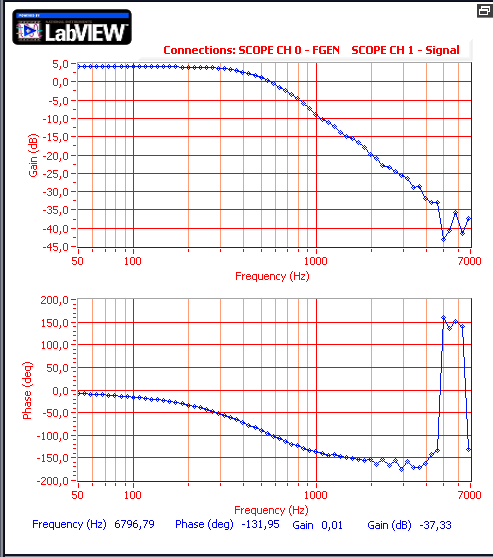
\includegraphics{obrazki/batman1.PNG}
\end{center}
\caption{filtr Butterwortha}
\end{figure}

\begin{figure}
\begin{center}
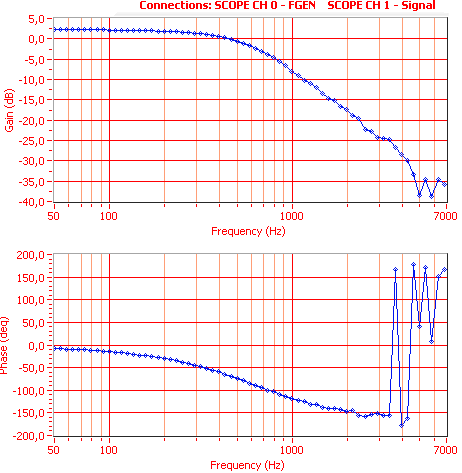
\includegraphics{obrazki/belzebub1bialy.png}
\end{center}
\caption{filtr Bessela}
\end{figure}

\begin{figure}
\begin{center}
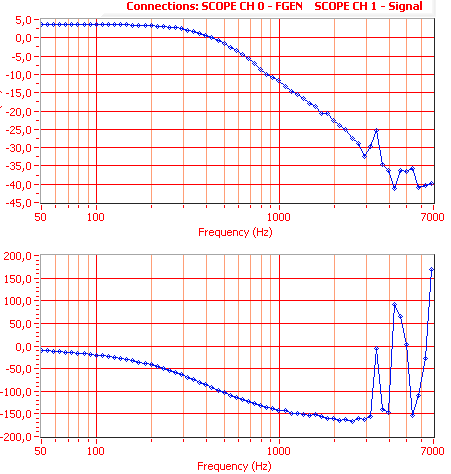
\includegraphics{obrazki/trzebieszow1bialy.png}
\end{center}
\caption{filtr Czebyszewa}
\end{figure}


Przydałoby się na te odpowiedzi dłużej popatrzeć i na przykład
pomocą systemowej linijki zmierzyć jaki jest spadek i czy wartości
pokrywają się nam z wyliczeniami.

Możemy też zasymulować te charakterystyki i pezpośrednio porównać,
gdybyśmy wykreślili wykresy od częstotliwości.

\section{Odpowiedzi na skok jednostkowy}


\begin{figure}
\begin{center}
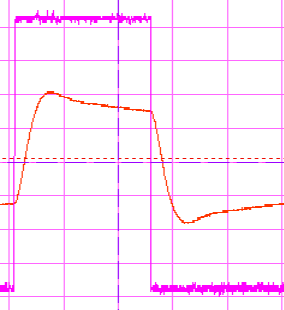
\includegraphics{obrazki/batman1prostybialymod.png}
\end{center}
\caption{filtr Butterwortha}
\end{figure}

\begin{figure}
\begin{center}
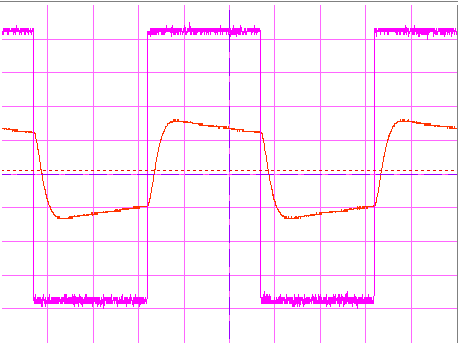
\includegraphics{obrazki/bezelprostybialy.png}
\end{center}
\caption{filtr Bessel'a}
\end{figure}

\begin{figure}
\begin{center}
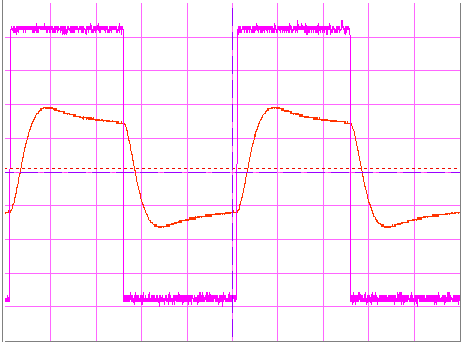
\includegraphics{obrazki/tszebieszowprostzbialy.png}
\end{center}
\caption{filtr Czebyszewa}
\end{figure}

\section{Projekt filtru}
\subsection{Obliczenia}
Obliczenia i wykreślone charakterystyki dołączamy jako osobny załącznik pod nazwą projekt filtru.

Znajdują się tam wszystkie niezbędne informacje.
\subsection{Zmierzona charakterystyka}

\begin{figure}
\begin{center}
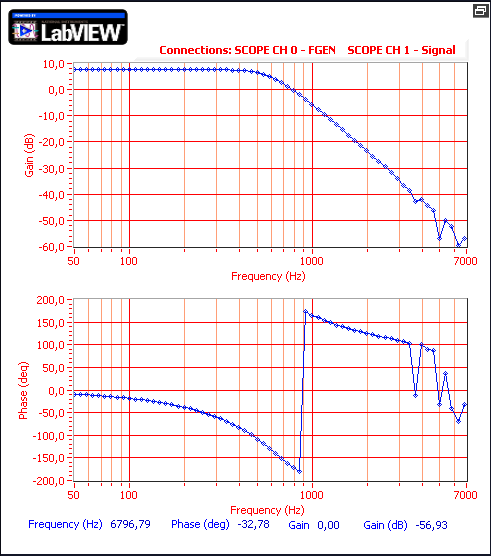
\includegraphics{obrazki/maslowilkcialobialy.png}
\end{center}
\caption{charakterystyka amplitudowa i fazowa filtru Butterworth'a trzeciego rzędu}
\end{figure}

\section{Opracowanie danych}

\section{Dyskusja niepewności}

\section{Wnioski}


Niech się dzieje zajebistość.

\end{document}